\documentclass[12pt,letter]{article}

%% \ifCLASSOPTIONcompsoc
%% % IEEE Computer Society needs nocompress option
%% % requires cite.sty v4.0 or later (November 2003)
%% \usepackage[nocompress]{cite}
%% \else
%% % normal IEEE
%% \usepackage{cite}
%% \fi

%% \usepackage[fleqn]{amsmath}
\usepackage[margin=1in]{geometry}
\usepackage{amsmath,amsfonts,amsthm,bm}
\usepackage{breqn}
\usepackage{amsmath}
\usepackage{amssymb}
\usepackage{tikz}
\usepackage{algorithm2e}
\usepackage{siunitx}
\usepackage{graphicx}
\usepackage{subcaption}
%% \usepackage{datetime}
\usepackage{multirow}
\usepackage{multicol}
\usepackage{mathrsfs}
\usepackage{fancyhdr}
\usepackage{fancyvrb}
\usepackage{parskip} %turns off paragraph indent
\pagestyle{fancy}

\usetikzlibrary{arrows}

\DeclareMathOperator*{\argmin}{argmin}
\newcommand*{\argminl}{\argmin\limits}

\newcommand{\mathleft}{\@fleqntrue\@mathmargin0pt}
\newcommand{\R}{\mathbb{R}}
\newcommand{\Z}{\mathbb{Z}}
\newcommand{\N}{\mathbb{N}}

\setcounter{MaxMatrixCols}{20}

\begin {document}

\rhead{(Bill) Yuan Liu, student \#: 996954078\\ Date: 2019/12/10}
\lhead{CSC2321F - Matrix Calculations - Assignment 3}

\begin{enumerate}
  
\item $u_{xxxx}+u=g$ where $u$ is periodic on $(a,b)$\\
  \begin{enumerate}
  \item
    Let $a=0,b=2\pi, n=6, u(x)=sin(x)$.\\
    Give $A$ and $\bar{g}$.\\
    \begin{align*}
      A & \leftarrow \frac{1}{h^4}Toeplitz(\begin{bmatrix}6 & -4 & 1 & 0 & 1 & -4\end{bmatrix})+I\\
      A(:,1) & \leftarrow A(:,1) * 2\\
      \\
      A= \frac{1}{h^4} &\begin{bmatrix}
        2 & & & & & \\
        & 1 & & & & \\
        & & 1 & & & \\
        & & & 1 & & \\
        & & & & 1 & \\
        & & & & & 1 \\
      \end{bmatrix}
      +
      \frac{1}{h^4}
      \begin{bmatrix}
        12 & -4 & 1 & 0 & 1 & 4\\
        -8 & 6 & -4 & 1 & 0 & 1\\
        2 & -4 & 6 & -4 & 1 & 0\\
        0 & 1 & -4 & 6 & -4 & 1\\
        2 & 0 & 1 & -4 & 6 & -4\\
        -8 & 2 & 0 & 1 & -4 & 6 \\
      \end{bmatrix}
      \\
      \bar{g_i}&=2 sin(\frac{2 \pi i}{6}), i=0,..,5\\      
    \end{align*}
    
    \pagebreak
    
  \item Adjust programme for assignment 1 to solve above with CG with tolerance $10^{-8}$ and zero vector as the initial guess\\
\begin{verbatim}
function [x,it] = mysolver(a, b, n, u, x)
% assumes u(x) is a symbolic function
    
    range = b-a;
    h = range/n;
    t = 0:1:n-1;
    xs = h.*t + a;
    
    g_symbol = diff(u,x,4) + u;
    g = eval(g_symbol(xs)');
    
    % construct A
    r = [6 -4 1 zeros(1,n-5) 1 -4];
    A = sparse(toeplitz(r));
    A=A./(h^4); % for u''''
    I=spdiags([ones(n)],0:0,n,n); %for u
    A=A+I;
    A(:,1) = A(:,1)*2; %for periodic boundary condition
    
    % solve with CG
    tol = 10^(-8);
    maxit = n;
    % x0 zero vector, preconditioner = I
    [x,flag,relres,iter] = pcg(A,g,tol,maxit,[],[],[]);
    it=iter;
end
\end{verbatim}
    
    \pagebreak
    
\begin{verbatim}
clear
% run solver for each dim for each case and record max knot errors

dims = [ 8 16 32 64 128 ];

% note: reset errors before running
errors = [];
iterations = [];

b = 2*pi;
a = 0;
range = b-a;

% case: u(x)=sin(x)
for e = 1:length(dims)

    n=dims(e);
    
    h = range/n;
    t = 0:1:n-1;
    xs = range/n.*t + a;
    
    syms u(x);
    u(x)=sin(x);

    [approx,iter] = mysolver(a, b, n, u, x);
    exact = eval(u(xs)');

    max_error_knots = 0;
    max_error_knots = max(max_error_knots, max(abs(approx-exact)));
    errors = [errors max_error_knots];
    iterations = [iterations iter];
    
    fprintf("case 1, n: %d, max knot error: %f, iterations: %d\n", n, max_error_knots, iter);
end
\end{verbatim}
    
    \pagebreak
    \begin{table}[h]
      \begin{center}
        \begin{tabular}{ | c | c | c |}
          \hline
          n & max absolute knot error & \# of iter for convergence\\
          \hline
          8 & 0.051625 & 1\\
          \hline
          16 & 0.012867 & 1\\
          \hline
          32 & 0.003214 & 1\\
          \hline
          64 & 0.000803 & 1\\
          \hline
          128 & 0.000201 & 1\\
          \hline
        \end{tabular}
        \caption{Error and Convergence}
      \end{center}
    \end{table}

    Solution $\bar{u}$ is a multiple of $\bar{g}$ for matrix $A$, then $u$ is a scaled eigenvector for A. Since preconditioner is $I$ and initial guess is the zero vector, the starting residual is $\bar{g}$ which is a multiple of the eigenvector. With conjugate gradient method, if the residual coincides with the direction vector that is generated at each iteration, then the next iteration converges. This is because CG algorithm is designed to get rid of error components in terms of a direction vector at each iteration. This explains in all cases of $n$, the number of iterations needed for convergence is 1.\\
    
  \end{enumerate}

  \pagebreak
  
\item Let A be $n \times n$, spd matrix
  Let A be a n $\times$ n symmetric positive definite matrix, and assume that the Conjugate Gradient (CG) method is applied to Ax = b, for some n × 1 vector b. Show that the direction vectors d (k) , and the residual vectors r (k) generated by the CG method satisfy:
  \begin{align*}
    r^{(k)} & \in span(d^{(0)} , d^{(1)} , . . . , d^{(k)} ), for\ k = 0, . . . , n − 1\\
    Ad^{(k)} & \in span(d^{(0)} , d^{(1)} , . . . , d^{(k+1)} ), for\ k = 0, . . . , n − 2
  \end{align*}
  and
  \begin{align*}
    span(d^{(0)} , d^{(1)} , . . . , d^{(k)} ) &= span(d^{(0)} , Ad^{(0)} , . . . , A^k d^{(0)} )\\
    &= span(r^{(0)} , Ar^{(0)} , . . . , A^k r^{(0)} ), for\ k = 0, . . . , n − 1
  \end{align*}
  By construction of CG algorithm and initial condition,
  \begin{align*}
    r^{(k)} &= r^{(k-1)}-\lambda_{k-1}Ad^{(k-1)}\\
    d^{(k)} &= r^{(k)}+\alpha_k d^{(k-1)}\\
    d^{(0)} &= r^{(0)}
  \end{align*}
  \begin{align*}
    &d^{(0)} = r^{(0)} \in span(d^{(0)})\\
    &\text{Assume } r^{(k)} \in span(d^{(0)}, ..., d^{(k)}) \text{ is true}\\
    \\
    &\text{From recursion of conjugate gradient:}\\
    &r^{(k+1)} \text{ is a linear combination of } r^{(k)}, Ad^{(k)} \implies\\
    &\text{\ \ \ \ \ \ \ \ } r^{(k+1)} \in span(d^{(0)}, ..., d^{(k)}, Ad^{(k)})\\
    &d^{(k+1)} \text{ is a linear combination of } r^{(k)}, d^{(k)}, Ad^{(k)} \implies\\
    &\text{\ \ \ \ \ \ \ \ } d^{(k+1)} \in span(r^{(k)}, d^{(k)}, Ad^{(k)}) = span(d^{(0)}, ..., d^{(k)}, Ad^{(k)})\\
    &\text{This means}\\
    &Ad^{(k)} \in span(d^{(0)}, ..., d^{(k)}, d^{(k+1)}), k=0,..,n-2\\
    \\
    &\text{Then}\\
    &r^{(k+1)} \in span(d^{(0)}, ..., d^{(k)}, Ad^{(k)})=span(d^{(0)}, ..., d^{(k)}, d^{(k+1)})\\
    &\text{thus completing induction, } r^{(k)} \in span(d^{(0)}, ..., d^{(k)}, d^{(k)}), k=0,..,n-1\\
  \end{align*}
  \begin{align*}
    &\text{Since CG is a CD method, by design d is A-orthogonal, } (d^{(i)},Ad^{(j)})=0, \forall i<j, \text{ then}\\
    &d^{(k+1)} \in span(d^{(0)}, ..., d^{(k)}, Ad^{(k)})=span(d^{(k)}, Ad^{(k)})\\
    &\text{recursive application results in}\\
    &d^{(1)} \in span(d^{(0)}, Ad^{(0)})\\
    &d^{(2)} \in span(d^{(1)}, Ad^{(1)})=span(d^{(0)}, Ad^{(0)}, A^2 d^{(0)}))\\
    &d^{(k)} \in span(d^{(k-1)}, A d^{(k-1)}) = span(d^{(0)},..., A^k d^{(0)})\\
    \\
    &d^{(i)} \in span(d^{(j)}),j>i\\
    \\
    &\text{Then}\\
    &span(d^{(0)}, ..., d^{(k)}) = span(d^{(0)}, Ad^{(0)}, ..., A^k d^{(0)})\\
    \\
    &\text{From earlier, since } d^{(k+1)}, r^{(k+1)} \in span(d^{(0)}, ..., d^{(k)}, d^{(k+1)}), \text{ then,}\\
    &d^{(k)} \text{ and } r^{(k)} \text{ lives in the same subspace at each iteration, thus:}\\
    &span(d^{(0)}, ..., d^{(k)}) = span(r^{(0)}, Ar^{(0)}, ..., A^k r^{(0)})\\
  \end{align*}
  
  \pagebreak
  
\item Let A be a n $\times$ n symmetric positive definite matrix, and assume that the CG method is applied to $Ax=b$, for some n $\times$ 1 vector b. Show that the CG iterate $x^{(k+1)}$ minimized $\|x-\hat{x}\|_{A^{\frac{1}{2}}}$ over all $\hat{x} \in x^{(0)} + span(d^{(0)}, ..., d^{(k)})$.\\

  Translation to linear space: $e^{(i)}=x^{(i)}-\hat{x}$, where $\hat{x}$ is the answer\\
  % $\|e^{(i)}\|_{A^{\frac{1}{2}}}^2=((A^{\frac{1}{2}}e^{(i)})^T,A^{\frac{1}{2}}e^{(i)})$\\
  % $\|e^{(i)}\|_{A^{\frac{1}{2}}}^2=e^{(i)}^T(A^{\frac{1}{2}})^T A^{\frac{1}{2}} e^{(i)} = e^{(i)}^T A e^{(i)}$ since $A$ is spd and $A^{\frac{1}{2}}$ is symmetric\\
  % $A$ is spd, then $e^{(i)}^T A e^{(i)}=0$ iff $e=0$, and this also minimizes $\|e^{(i)}\|_{A^{\frac{1}{2}}}$\\
  Using CG algorithm to reduce $e$:\\
  let $e^{(0)}=\sum_{i=0}^{n-1} c_i d^{(i)}$\\
  $Ae^{(0)}=\sum_{i=0}^{n-1} c_i A d^{(i)}$\\
  $(d^{(k)},Ae^{(0)})=\sum_{i=0}^{n-1} c_i (d^{(k)},A d^{(i)})$\\
  Using A-orthogonality of d vectors: $(d^{(k)},Ad^{(i)})=0, k<i$, $c_k$ is chosen such that:\\
  $(d^{(k)},Ae^{(0)})= c_k (d^{(k)},A d^{(k)})$\\
  $c_k= \frac{(d^{(k)},Ae^{(0)})}{(d^{(k)},Ad^{(k)})}$\\
  $c_k= \frac{(d^{(k)}, A(e^{(0)} + \sum_{i=0}^{k-1} - \frac{(d^{(i)},Ae^{(i)})}{(d^{(i)},Ad^{(i)})} d^{(i)}))}{{(d^{(k)},Ad^{(k)})}}$ since $d$ vectors are A-orthogonal\\
  From CG algorithm: $x^{(i+1)} = x^{(i)} - \frac{(d^{(i)},Ae^{(i)})}{(d^{(i)},Ad^{(i)})} d^{(i)}$:\\
  $c_k= \frac{(d^{(k)}, Ae^{(k)})}{{(d^{(k)},Ad^{(k)})}}$\\
  $x^{(i+1)} = x^{(i)} - c_k d^{(i)}$\\
  $e^{(i)}=e^{(0)}-\sum_{j=0}^{i-1}c_j d^{(j)}$ which eliminiates a component of the error at each iteration\\
  By the end of all iterations, $e^{(n-1)}=e^{(0)}-\sum_{j=0}^{n-1}c_j d^{(j)}=0$\\
  At each iteration, component $d^{(i)}$ of $e^{(0)}$ is reduced to 0.\\
  With A-orthogonality, components $d^{(j)}, j \in 0,..,i$ of $e$ are reduced to 0 and stays at 0 after iteration $i$, thus satisfying minimization of $\|e=x-\hat{x}\|$ in $span(d^{(0)}, ..., d^{(i)})$ after each iteration i.\\
  
  \pagebreak
  
\item
  
  Generalizing for assignment 2 question 3 and modifying boundary condition:\\
  \begin{align*}
    au_{xxxx} + bu_{xxyy} + cu_{yyyy} + du_{xx} + eu_{yy} + f u & = g\\
    u & = \gamma\\
    u_{xx} & =\zeta\\
    u_{y} & =\eta\\
  \end{align*}

  \begin{enumerate}
  \item For $a=1,b=2,c=1,d=0,e=0,f=0$, modify algorithm from assignment 2 question to handle modified boundary condition.\\

    Using method of undetermined coefficients for the new $u_y$ boundary condition:\\

    At $y=0 (j=0)$:
    \begin{align*}
      a_{-1} u_{i,j-1} & = a_{-1}(u_{i,j}+u_{i,j}^{(1)}(-h)+ \frac{u_{i,j}^{(2)}(-h)^2}{2!} + \frac{u_{i,j}^{(3)}(-h)^3}{3!} + \frac{u_{i,j}^{(4)}(-h)^4}{4!}) + o(h^5)\\
      a_{0} u_{i,j} & = a_{0} u_{i,j}\\
      a_{1} u_{i,j+1} & = a_{1}(u_{i,j}+u_{i,j}^{(1)}(h)+ \frac{u_{i,j}^{(2)}(h)^2}{2!} + \frac{u_{i,j}^{(3)}(h)^3}{3!} + \frac{u_{i,j}^{(4)}(h)^4}{4!}) + o(h^5)\\
      a_{2} u_{i,j+2} & = a_{2}(u_{i,j}+u_{i,j}^{(1)}(2h)+ \frac{u_{i,j}^{(2)}(2h)^2}{2!} + \frac{u_{i,j}^{(3)}(2h)^3}{3!} + \frac{u_{i,j}^{(4)}(2h)^4}{4!}) + o(h^5)\\
      a_{2} u_{i,j+3} & = a_{3}(u_{i,j}+u_{i,j}^{(1)}(3h)+ \frac{u_{i,j}^{(2)}(3h)^2}{2!} + \frac{u_{i,j}^{(3)}(3h)^3}{3!} + \frac{u_{i,j}^{(4)}(3h)^4}{4!}) + o(h^5)
    \end{align*}
    
    Solve:\\
    
    $
    \begin{bmatrix}
      1 & 1 & 1 & 1 & 1\\
      -1 & 0 & 1 & 2 & 3\\
      1 & 0 & 1 & 4 & 9\\
      -1 & 0 & 1 & 8 & 27\\
      1 & 0 & 1 & 16 & 81\\
    \end{bmatrix}
    \begin{bmatrix}
      a_{-1}\\
      a_{0}\\
      a_{1}\\
      a_{2}\\
      a_{3}\\
    \end{bmatrix}=
    \begin{bmatrix}
      0\\
      1\\
      0\\
      0\\
      0\\
    \end{bmatrix}
    $\\

    $
    \begin{bmatrix}
      a_{-1}\\
      a_{0}\\
      a_{1}\\
      a_{2}\\
      a_{3}\\
    \end{bmatrix}=
    \begin{bmatrix}
      -1/4\\
      -5/6\\
      3/2\\
      -1/2\\
      5/60\\
    \end{bmatrix}
    $\\

    \pagebreak
    
    Stencil centered at $j=0$:\\
    $\eta=
    \frac{1}{h}
    \begin{bmatrix}
      & & \frac{5}{60} & & \\
      & & -\frac{1}{2} & &\\
      & & \frac{3}{2} & &\\
      & & -\frac{5}{6} & &\\
      & & -\frac{1}{4} & & \\
      & & 0 & & \\
      & & 0 & & \\
    \end{bmatrix}
    +o(h^4)$\\
    
    At $y=1 (j=n)$:
    \begin{align*}
      a_{+1} u_{i,j+1} & = a_{+1}(u_{i,j}+u_{i,j}^{(1)}(h)+ \frac{u_{i,j}^{(2)}(h)^2}{2!} + \frac{u_{i,j}^{(3)}(h)^3}{3!} + \frac{u_{i,j}^{(4)}(h)^4}{4!}) + o(h^5)\\
      a_{0} u_{i,j} & = a_{0} u_{i,j}\\
      a_{-1} u_{i,j-1} & = a_{-1}(u_{i,j}+u_{i,j}^{(1)}(-h)+ \frac{u_{i,j}^{(2)}(-h)^2}{2!} + \frac{u_{i,j}^{(3)}(-h)^3}{3!} + \frac{u_{i,j}^{(4)}(-h)^4}{4!}) + o(h^5)\\
      a_{-2} u_{i,j-2} & = a_{-2}(u_{i,j}+u_{i,j}^{(1)}(-2h)+ \frac{u_{i,j}^{(2)}(-2h)^2}{2!} + \frac{u_{i,j}^{(3)}(-2h)^3}{3!} + \frac{u_{i,j}^{(4)}(-2h)^4}{4!}) + o(h^5)\\
      a_{-3} u_{i,j-3} & = a_{-3}(u_{i,j}+u_{i,j}^{(1)}(-3h)+ \frac{u_{i,j}^{(2)}(-3h)^2}{2!} + \frac{u_{i,j}^{(3)}(-3h)^3}{3!} + \frac{u_{i,j}^{(4)}(-3h)^4}{4!}) + o(h^5)
    \end{align*}
    
    Solve:\\
    
    $
    \begin{bmatrix}
      1 & 1 & 1 & 1 & 1\\
      1 & 0 & -1 & -2 & -3\\
      1 & 0 & 1 & 4 & 9\\
      -1 & 0 & -1 & -8 & -27\\
      1 & 0 & 1 & 16 & 81\\
    \end{bmatrix}
    \begin{bmatrix}
      a_{+1}\\
      a_{0}\\
      a_{-1}\\
      a_{-2}\\
      a_{-3}\\
    \end{bmatrix}=
    \begin{bmatrix}
      0\\
      1\\
      0\\
      0\\
      0\\
    \end{bmatrix}
    $\\

    $
    \begin{bmatrix}
      a_{+1}\\
      a_{0}\\
      a_{-1}\\
      a_{-2}\\
      a_{-3}\\
    \end{bmatrix}=
    \begin{bmatrix}
      1/4\\
      5/6\\
      -3/2\\
      1/2\\
      -5/60\\
    \end{bmatrix}
    $\\
    
    Stencil centered at $j=n$:\\
    $\eta=
    \frac{1}{h}
    \begin{bmatrix}
      & & 0 & & \\
      & & 0 & & \\
      & & \frac{1}{4} & & \\
      & & \frac{5}{6} & &\\
      & & -\frac{3}{2} & &\\
      & & \frac{1}{2} & &\\
      & & -\frac{5}{60} & & \\
    \end{bmatrix}
    +o(h^4)$\\
    
    Original boundary condition stencil applied from assignment 2 question 3 centered at $j=n$ and $j=0$:\\
    
    $ -\frac{1}{h^2}\eta_{orig} = \frac{1}{h^4}
    \begin{bmatrix}
      & &  0  & & \\
      & & -1  & & \\
      & &  2  & & \\
      & &  -1  & & \\
      & &  0  & & \\
    \end{bmatrix}+o(1)$\\
    
    With original coefficient matrix, unapply original boundary stencil of $u_{yy}$ and apply new boundary stencil of $u_y$ onto the coefficient matrix:\\

    At $j=0$:\\
    
    $\frac{1}{h^2}\eta_{orig} + \frac{4}{h^3} \eta_{new}=
    \frac{1}{h^4}
    \begin{bmatrix}
      & & \frac{1}{3} & & \\
      & & -2 & &\\
      & & 1+6 & &\\
      & & -2-\frac{10}{3} & &\\
      & & 1-1 & & \\
      & & 0 & & \\
      & & 0 & & \\
    \end{bmatrix}
    $\\

    At $j=n$:\\
    
    $\frac{1}{h^2}\eta_{orig} - \frac{4}{h^3} \eta_{new}=
    \frac{1}{h^4}
    \begin{bmatrix}
      & & 0 & & \\
      & & 0 & & \\
      & & 1-1 & & \\
      & & -2-\frac{10}{3} & &\\
      & & 1+6 & &\\
      & & -2 & &\\
      & & \frac{1}{3} & & \\
    \end{bmatrix}
    $\\

    \pagebreak
    
    Changes applied to interior grid affecting each column of the grid:\\
    \begin{align*}
    \begin{bmatrix}
      7\\
      -2\\
      \frac{1}{3}\\
      0\\
      ...\\
      0\\
      \frac{1}{3}\\
      -2\\
      7\\
    \end{bmatrix}
    \end{align*}\\
    
    This results in a delta ($C$) to the block diagonals of the coefficient matrix corresponding for each column as on top of the original values:\\
    
    $C = 
    \begin{bmatrix}
      7 & -2 & \frac{1}{3} & 0 & ... & &\\
      0 & ... & & & & &\\
      & & & & & &\\
      & & & & ... & & 0 \\
      & & ... & 0 &\frac{1}{3} & -2 & 7\\
    \end{bmatrix}
    $\\

    Overall delta to the coefficient matrix is $I_{n-1} \otimes C$\\

    Boundary value constants moved to the RHS of the equation, Ax=g, for the changed boundary condition:\\
    
    $j=1$:\\
    $-\frac{1}{h^4}(\frac{-16}{3}\gamma_{i,0}+2\gamma_{i-1,0}+2\gamma_{i+1,0})+\frac{4}{h^3} \eta_{new}$\\

    $j=n-1$:\\
    $-\frac{1}{h^4}(\frac{-16}{3}\gamma_{i,n}+2\gamma_{i-1,n}+2\gamma_{i+1,n})-\frac{4}{h^3} \eta_{new}$\\

    Reset of procedures is unchanged from the original problem.\\
    
    \pagebreak
    
    Block diagonalization is modified by adding the change of the coefficient matrix represented by $C$.\\
  
  $A=\frac{1}{h^4}(I_{n-1} \otimes tri\{1,-2,1\}^2 + tri\{1,-2,1\}^2 \otimes I_{n-1}+
  2\ tri\{1,-2,1\} \otimes tri\{1,-2,1\}+I_{n-1} \otimes C)$\\

  let $T=tri\{1,-2,1\}$\\
  
  let $V$ be a matrix of eigenvectors of $tri\{1,-2,1\}$\\
  let $V^{-1}TV=D_T$ be diagonalization of $tri\{1,-2,1\}$\\
  $D_T=diag(-4 sin^2(\frac{l \pi}{2n})), l = 1,..,n-1$\\
  let $(V^{-1}TV)^2=V^{-1}T^2 V=D_T^2=D_B$ be diagonalization of matrix $(tridiag\{1,-2,1\})^2$
  \begin{align*}
    I = & I_{n-1}\\
    Block=&(V^{-1} \otimes I^{-1})A(V \otimes I)\\
    Block=&(V^{-1} \otimes I^{-1})(\frac{1}{h^4}(I \otimes T^2 + T^2 \otimes I +2\ T \otimes T + I \otimes C ))(V \otimes I)\\    
    Block=&\frac{1}{h^4}((V^{-1} \otimes I^{-1})(I \otimes T^2)(V \otimes I)\\
          &+(V^{-1} \otimes I^{-1})(T^2 \otimes I)(V \otimes I)\\
          &+(V^{-1} \otimes I^{-1})(2\ T \otimes T)(V \otimes I))\\
          &+(V^{-1} \otimes I^{-1})(I_{n-1} \otimes C)(V \otimes I))\\
    Block=&\frac{1}{h^4}((V^{-1}IV)\otimes(I^{-1}T^2I)\\
          &+(V^{-1}T^2V)\otimes(I^{-1}II)\\
          &+2(V^{-1}TV)\otimes(I^{-1}TI))\\
          &+((V^{-1}IV)\otimes(I^{-1} C I)\\
    Block=&\frac{1}{h^4}(I\otimes T^2 + D_B \otimes I +2(D_T \otimes T ) + I \otimes C)\\
  \end{align*}

  \pagebreak
  
  FFT based procedure to solve u, from assignment 2, problem 3:\\

  $A=(V \otimes I)Block(V^{-1} \otimes I^{-1})$\\
  $A^{-1}=(V \otimes I)Block^{-1}(V^{-1} \otimes I^{-1})$\\
  $\bar{u}=A^{-1}\bar{g}=(V \otimes I)Block^{-1}(V^{-1} \otimes I)\bar{g}$\\
  $\bar{u}=(\bold{F}^{-1} \otimes I)Block^{-1}(\bold{F} \otimes I)\bar{g}$\\

  DST of size $n-1$ to each column of $\bar{g}_{m-1 \times n-1}^T$:\\
  $\bar{g}_{m-1 \times x-1}=reshape(\bar{g},[m-1,n-1])$\\
  $\bar{g}_{m-1 \times n-1}^{(1)}= (dst(\bar{g}_{m-1 \times x-1}^T))^T$\\
  $stack(\bar{g}_{m-1,n-1}^{(1)}) = (\bold{F} \otimes I) \bar{g}$\\
  
  solve $B \bar{g}^{(2)} = stack(\bar{g}_{m-1,n-1}^{(1)})$ for $\bar{g}^{(2)}$ via block solver:\\
  $\bar{g}^{(2)}=B \backslash stack(\bar{g}_{m-1,n-1}^{(1)})$\\
  
  inverse DST of size $n-1$ to each column of $(\bar{g}_{m-1,n-1}^{(2)})^T$:\\
  $\bar{g}_{m-1.n-1}^{(2)}=reshape(\bar{g}^{(2)},[m-1,n-1])$\\
  $u_{m-1,n-1}=(idst((\bar{g}_{m-1,n-1}^{(2)})^T))^T$\\
  $\bar{u}=stack(u_{m-1,n-1})=(\bold{F}^{-1} \otimes I^{-1}) \bar{g}^{(2)}$\\

  \pagebreak
  
\item Write program for the generalized problem.\\

\begin{verbatim}
function [u_gmres,flag,relres,iter,resvec,A,g] = solver_pgmres(n,u,x,y,...
                                                     a,b,c,d,e,f)
%assume u(x,y),a,b,c,d,e,f are symbolic functions

dim=n-1;
h=1/n;

%a u_xxxx + b u_xxyy + c u_yyyy + d u_xx + e u_yy + f u = g

u_xxxx = diff(u,x,4);
u_yyyy = diff(u,y,4);
u_xxyy = diff(diff(u,x,2),y,2);
u_xx = diff(u,x,2);
u_yy = diff(u,y,2);

%boundary values
eta = sym('eta');
zeta = sym('zeta');

eta = diff(u,y,1);
zeta = diff(u,x,2);

gamma = sym('gamma');
gamma = u;

g = sym('g');
g(x,y) = a(x,y) * u_xxxx(x,y) + b(x,y) * u_xxyy(x,y) + c(x,y) * u_yyyy +...
         d(x,y) * u_xx(x,y) + e(x,y) * u_yy(x,y) + f(x,y) * u(x,y);

[A,g] = create_A_g_generic(n,x,y,a,b,c,d,e,f,g,...
    u_xxxx,u_xxyy,u_yyyy,u_xx,u_yy,eta,zeta,gamma);

%solver: gmres
maxit = 50;
tol = 10^(-9);
restart = 20;

[ret_u,ret_flag,ret_relres,ret_iter,resvec] = gmres(A,g,restart,tol,...
                                                    maxit,@precond);

u_gmres = ret_u;
flag = ret_flag;
relres = ret_relres;
iter = ret_iter;

    function u_solve = precond(r)
        h = 1/n;
        dim = n-1;
        [AA, B, T, C] = create_A_2(n);
        % use r from input instead of generating g vector
        % f_eta = diff(u,y,1);
        % f_zeta = diff(u,x,2);
        % %compute boundary values
        % g2 = compute_boundary_value_constants_2(n,f,f_eta,f_zeta);
        % %compute g(4th order mixed derivatives) on interior grid points
        % f_4th = diff(u,x,4) + 2*diff(diff(u,x,2), y, 2) + diff(u,y,4);
        % g1_grid = compute_grid(n,f_4th,x,y);
        % assert((size(g1_grid,1)==n-1) && (size(g1_grid,2)==n-1));
        % %remap grid points to 1D matrix
        % g1 = zeros(n-1*n-1,1);
        % for i=1:n-1
        %     for j=1:n-1
        %         g1(ij_to_k(dim, i, j),1)=g1_grid(i, j);
        %     end
        % end
        % g = g1+g2;
        %%%%%%%%%%%%%%%%%%%%%%%%%%%%
        % dst + block LU solver:
        % equivalent to:
        %     u = kron(F^-1_n, I_m) BlockDiag^-1 kron(F_n,I_m)g
        %     BlockDiag := block diagonalization of A

        I = eye(dim);
        j = 1:1:n-1;
    
        %compute eigenvalues of tridiag{1,-2,1}
        eigenvalues = -4*(sin(j*pi/(2*n))).^2;
        D_T = spdiags(eigenvalues', 0:0, dim, dim);
        % alternative: use eigs
        % need to reverse order to match up with ordering of dst, idst
        %D_T = spdiags([flip(eigs(T,dim))], 0:0, dim, dim); %alternative
    
        % kron(I,C) added below for the augmentation of 
        % changed boundary condition from u_yy to u_y
        D_B = D_T^2;
        BlockDiag = (1/h^4)*(kron(I,T*T)+...
                             kron(D_B,I)+...
                             2*(kron(D_T,T))+...
                             kron(I,C));

        %shape g to m by n matrix, 
        %m being y-axis (fastest increasing axis)
        %of original grid
        g_m_by_n = reshape(r,[dim,dim]);
        %transform by eigenvectors
        g_1_n_by_m = dst(g_m_by_n');
        g_1_stacked = reshape(g_1_n_by_m',[dim*dim,1]);
        %solve BlockDiag g_2 = g_1
        g_2_stacked = BlockDiag\g_1_stacked;
        g_2_m_by_n = reshape(g_2_stacked, [dim, dim]);
        %inverse transform by eigenvectors
        u_n_by_m = idst(g_2_m_by_n');
        u_solve = reshape(u_n_by_m',[dim*dim,1]);
        %%%%%%%%%%%%%%%%%%%%%%%%%%%
    end
end
\end{verbatim}

\pagebreak

\begin{verbatim}
function [A, B, T, C] = create_A_2(n)
    
    h=1/n;
    dim = n-1;
    I = eye(dim);

    %using composition of operators: u_xxxx+u_yyyy+2u_xxyy = (u_xx+u_yy)^2

    %construct tridiagonal matrix used for u_xx, u_yy
    %for each of dimensions x,y
    T = spdiags([ones(dim,1) -2*ones(dim,1) ones(dim,1)],...
                -1:1,...
                dim,dim);

    %let fastest increasing index to be along y dimension
    %kronecker product corresponding to difference operator u_yy
    B_yy = kron(I,T);
    %kronecker product corresponding to difference operator u_xx
    B_xx = kron(T,I);

    %matrix corresponding to (u_xx+u_yy)
    B = B_yy + B_xx;
    
    %alter values near boundary due to change of boundary condition
    %from u_yy = eta to u_y = eta
    C = spdiags([zeros(dim,1)], 0:0, dim, dim);

    %here we change matrix to revert origin boundary condition
    %corresponding to u_yy and apply the new boundary condition 
    %for u_y
    %apply 4 * eta B.C. at bottom (j=1)
    %apply -4 * eta B.C. at top (j=n-1)
    D_bottom = 4*[-1/4 -5/6 3/2 -1/2 5/60];
    D_top = -4*flip([1/4 5/6 -3/2 1/2 -5/60]);
    
    C(1,1) = 1; %revert old boundary condition in y direction
    %apply new u_y boundary condition at j=1
    C(1,1:3) = C(1,1:3) + D_bottom(3:5);
    C(dim,dim) = 1; %revert old boundary condition in y direction
    %apply new u_y boundary condition at j=n-1
    C(dim,dim-2:dim) = C(dim,dim-2:dim) + D_top(1:3);

    CC = kron(I,C);
    A = 1/(h^4) * (CC + B^2);
end
\end{verbatim}

\pagebreak

\begin{verbatim}
function g2 = compute_boundary_value_constants_2(n,gamma,eta,zeta)
%compute boundary constants that touches or goes out of grid for
%the right hand side of Au=g
%returns negated value to be used for right side

%assumes gamma, eta, zeta are symbolic functions
%gamma: 0th order boundary condition
%eta: 1st order boundary condition along y dimension
%zeta: 2nd order boundary condition along x dimension

dim = n-1;
h = 1/n;

g2 = zeros(dim*dim,1);

for i = 1:n-1
    for j = 1:n-1

        if ( (3<=i) && (i<= n-3) && (3<=j) && (j<= n-3))
            continue;
        end
        
        if (i==1)
            g2(ij_to_k(dim,i,j)) = g2(ij_to_k(dim,i,j))...
                                    -1/(h^4)*(+2*gamma(0,(j-1)*h)...
                                              -6*gamma(0,j*h)...
                                              +2*gamma(0,(j+1)*h))...
                                    -1/(h^2)*(zeta(0,j*h));
        elseif (i==2)
            g2(ij_to_k(dim,i,j)) = g2(ij_to_k(dim,i,j))...
                                    -1/(h^4)*(gamma(0,j*h));
        end
        
        if (i==n-1)
            g2(ij_to_k(dim,i,j)) = g2(ij_to_k(dim,i,j))...
                                    -1/(h^4)*(+2*gamma(1,(j-1)*h)...
                                              -6*gamma(1,j*h)...
                                              +2*gamma(1,(j+1)*h))...
                                    -1/(h^2)*(zeta(1,j*h));
        elseif (i==n-2)
            g2(ij_to_k(dim,i,j))= g2(ij_to_k(dim,i,j))...
                                    -1/(h^4)*(gamma(1,j*h));
        end
        
        if (j==1)
            %apply o(h^4) accuracy u_y BC: 
            % 4*eta/h^3 = +4*[-1/4 -5/6 3/2 -1/2 -5/60]*(1/h^4), 
            % where 4*-5/6=-10/3 is the boundary entry
            g2(ij_to_k(dim,i,j)) = g2(ij_to_k(dim,i,j))...
                                    -1/(h^4)*(+2*gamma((i-1)*h,0)...
                                              +(-8-10/3)*gamma(i*h,0)...
                                              +2*gamma((i+1)*h,0))...
                                    +4/(h^3)*(eta(i*h,0));
        elseif (j==2)
            g2(ij_to_k(dim,i,j)) = g2(ij_to_k(dim,i,j))...
                                    -1/(h^4)*(gamma(i*h,0));
        end

        if (j==n-1)
            %apply o(h^4) accuracy u_y BC:
            % -4*eta/h^3 = -4*flip([1/4 5/6 -3/2 1/2 -5/60])*(1/h^4), 
            % where -4*5/6=-10/3 is the boundary entry
            g2(ij_to_k(dim,i,j)) = g2(ij_to_k(dim,i,j))...
                                    -1/(h^4)*(+2*gamma((i-1)*h,1)...
                                              +(-8-10/3)*gamma(i*h,1)...
                                              +2*gamma((i+1)*h,1))...
                                    -4/(h^3)*(eta(i*h,1));
        elseif (j==n-2)
            g2(ij_to_k(dim,i,j)) = g2(ij_to_k(dim,i,j))...
                                    -1/(h^4)*(gamma(i*h,1));
        end
    end
end

%take care of overlap in corners in previous loops
g2(ij_to_k(dim,1,1)) = g2(ij_to_k(dim,1,1)) + 1/(h^4)*(2*gamma(0,0));
g2(ij_to_k(dim,1,n-1)) = g2(ij_to_k(dim,1,n-1)) + 1/(h^4)*(2*gamma(0,1));
g2(ij_to_k(dim,n-1,1)) = g2(ij_to_k(dim,n-1,1)) + 1/(h^4)*(2*gamma(1,0));
g2(ij_to_k(dim,n-1,n-1)) = g2(ij_to_k(dim,n-1,n-1)) + 1/(h^4)*(2*gamma(1,1));
\end{verbatim}

\pagebreak

\begin{verbatim}
function [A, rhs] = create_A_g_generic(n,x,y,a,b,c,d,e,f,g,...
                                       u_xxxx,u_xxyy,u_yyyy,...
                                       u_xx,u_yy,eta,zeta,gamma)
    %assumes a,b,c,d,e,f,u_xxxx,u_xxyy,u_yyyy,u_xx,u_yy are symbolic
    %a u_xxxx + b u_xxyy + c u_yyyy + d u_xx + e u_yy + f u = g
    
    h=1/n;
    dim = n-1;
    
    %padd 4 in each direction so that values at boundary and 1 grid outside
    %of boundary are captured
    pad = 4;
    pad_offset = 2;
    dim_mod = dim+4;
    
    rhs = sparse(zeros(dim_mod*dim_mod,1));

    gamma_aug = zeros(dim_mod,dim_mod);
    
    aa = zeros(dim,dim);
    bb = zeros(dim,dim);
    cc = zeros(dim,dim);
    dd = zeros(dim,dim);
    ee = zeros(dim,dim);
    ff = zeros(dim,dim);
    gg = zeros(dim,dim);
    
    for i=1:n-1
        for j=1:n-1
            aa(i,j) = double(a(i*h,j*h));
            bb(i,j) = double(b(i*h,j*h));
            cc(i,j) = double(c(i*h,j*h));
            dd(i,j) = double(d(i*h,j*h));
            ee(i,j) = double(e(i*h,j*h));
            ff(i,j) = double(f(i*h,j*h));
            gg(i,j) = double(g(i*h,j*h));
        end
    end
    
    aa_aug = zeros(dim_mod,dim_mod);
    bb_aug = zeros(dim_mod,dim_mod);
    cc_aug = zeros(dim_mod,dim_mod);
    dd_aug = zeros(dim_mod,dim_mod);
    ee_aug = zeros(dim_mod,dim_mod);
    ff_aug = zeros(dim_mod,dim_mod);
    gg_aug = zeros(dim_mod,dim_mod);
    
    for i=1:n-1
       aa_aug(:,2+i) = [ 0; 0; aa(:,i); 0; 0];
       bb_aug(:,2+i) = [ 0; 0; bb(:,i); 0; 0];
       cc_aug(:,2+i) = [ 0; 0; cc(:,i); 0; 0];
       dd_aug(:,2+i) = [ 0; 0; dd(:,i); 0; 0];
       ee_aug(:,2+i) = [ 0; 0; ee(:,i); 0; 0];
       ff_aug(:,2+i) = [ 0; 0; ff(:,i); 0; 0];
       gg_aug(:,2+i) = [ 0; 0; gg(:,i); 0; 0];
    end
    
    eta_eval = zeros(dim_mod,dim_mod);
    zeta_eval = zeros(dim_mod,dim_mod);
    
    for i=1:n-1+2
        point = (i-1)*h;
        eta_eval(i+1,2) = eta(point,0);
        eta_eval(i+1,dim_mod-1) = eta(point,1);
        
        zeta_eval(2,i+1) = zeta(0,point);
        zeta_eval(dim_mod-1,i+1) = zeta(1,point);
        
        gamma_aug(i+1,2) = gamma(point,0);
        gamma_aug(i+1,dim_mod-1) = gamma(point,1);
        gamma_aug(2,i+1) = gamma(0,point);
        gamma_aug(dim_mod-1,i+1) = gamma(1,point);
    end
    
    %stack by column (y-direction increasing fastest)
    aa_stack = sparse(reshape(aa_aug',[dim_mod*dim_mod,1]));
    bb_stack = sparse(reshape(bb_aug',[dim_mod*dim_mod,1]));
    cc_stack = sparse(reshape(cc_aug',[dim_mod*dim_mod,1]));
    dd_stack = sparse(reshape(dd_aug',[dim_mod*dim_mod,1]));
    ee_stack = sparse(reshape(ee_aug',[dim_mod*dim_mod,1]));
    ff_stack = sparse(reshape(ff_aug',[dim_mod*dim_mod,1]));
    gg_stack = sparse(reshape(gg_aug',[dim_mod*dim_mod,1]));
    
    eta_stack = sparse(reshape(eta_eval',[dim_mod*dim_mod,1]));
    zeta_stack = sparse(reshape(zeta_eval',[dim_mod*dim_mod,1]));
    
    gamma_stack = sparse(reshape(gamma_aug',[dim_mod*dim_mod,1]));
    
    op = ones(dim_mod,1);
    op_mod = ones(dim_mod,1);
    op_mod(1:2,1)=0;
    op_mod(dim_mod-1:dim_mod,1)=0;
    
    %u_xxxx block pentadiag [. . . . .]
    T = spdiags([op -4*op 6*op -4*op, op],...
                  -2:2,...
                  dim_mod,dim_mod);
    T(1:2,:)=0;
    T(dim_mod-1:dim_mod,:)=0;
    
    Txxxx = kron(T, diag(op_mod));

    %u_yyyy pentadiag [.....]
    T = spdiags([op -4*op 6*op -4*op, op],...
                  -2:2,...
                  dim_mod,dim_mod);
    T(1:2,:)=0;
    T(dim_mod-1:dim_mod,:)=0;
    
    Tyyyy = kron(diag(op_mod), T);

    %u_xxyy:
    T = spdiags([-2*op, 4*op, -2*op],...
                  -1:1,...
                  dim_mod,dim_mod);
    T(1:2,:)=0;
    T(dim_mod-1:dim_mod,:)=0;
    Txxyy_a = kron(diag(op_mod), T); %same column

    T = spdiags([op -2*op op],...
                  -1:1,...
                  dim_mod,dim_mod);
    T(1:2,:)=0;
    T(dim_mod-1:dim_mod,:)=0;

    II = spdiags([op],...
                  1,...
                  dim_mod,dim_mod);
    II(1:2,:)=0;
    II(end-1:end,:)=0;
    Txxyy_b = kron(II, T); %column to the right

    II = spdiags([op],...
                  -1,...
                  dim_mod,dim_mod);
    II(1:2,:)=0;
    II(end-1:end,:)=0;
    Txxyy_c = kron(II, T); %column to the left

    Txxyy = Txxyy_a + Txxyy_b + Txxyy_c;
    
    %u_xx tridiag [. . .]
    T = spdiags([op -2*op op],...
                  -1:1,...
                  dim_mod,dim_mod);
    T(1:2,:)=0;
    T(dim_mod-1:dim_mod,:)=0;
    Txx = kron(T, diag(op_mod));

    %u_yy tridiag [...]
    T = spdiags([op -2*op op],...
                  -1:1,...
                  dim_mod,dim_mod);
    T(1:2,:)=0;
    T(dim_mod-1:dim_mod,:)=0;
    Tyy = kron(diag(op_mod), T);

    %u
    T = spdiags([op],...
                 0,...
                 dim_mod,dim_mod);
    T(1:2,:)=0;
    T(dim_mod-1:dim_mod,:)=0;
    Tu = kron(diag(op_mod),T);

    %multiply by provided coefficients a,b,c,d,e,f
    %a u_xxxx + b u_xxyy + c u_yyyy + d u_xx + e u_yy + f u = g
    Txxxx_scaled = bsxfun(@times,Txxxx,aa_stack);
    Txxyy_scaled = bsxfun(@times,Txxyy,bb_stack);
    Tyyyy_scaled = bsxfun(@times,Tyyyy,cc_stack);
    Txx_scaled = bsxfun(@times,Txx,dd_stack);
    Tyy_scaled = bsxfun(@times,Tyy,ee_stack);
    Tu_scaled = bsxfun(@times,Tu,ff_stack);
    
    %gamma_stack contains the values at boundary, dot product with each row
    %to get boundary constants, move to right hand side of equation
    rhs = rhs - 1/(h^4)*(Txxyy_scaled * gamma_stack);
    rhs = rhs - 1/(h^2)*(Txx_scaled * gamma_stack);
    rhs = rhs - 1/(h^2)*(Tyy_scaled * gamma_stack);
    rhs = rhs - (Tu_scaled * gamma_stack);
    
    %cancel value outside of grid for boundary condition in x-direction:
    %Txxxx_scaled(:,1:dim_mod)
    %Txxxx_scaled(:,dim_mod*dim_mod-dim_mod+1:dim_mod*dim_mod)
    Tboundary_x = [1 -2 1];
    for row=1:dim_mod*dim_mod
        for i=1:dim_mod
            val = Txxxx_scaled(row,i);
            if val ~= 0
                val_negate = -val;
                scale = val_negate/Tboundary_x(1);
                rhs(row) = rhs(row) + scale * 1/(h^2) * zeta_stack(i+dim_mod);
                Tboundary_x_scaled = scale.* Tboundary_x;
                for j=1:length(Tboundary_x_scaled)
                    Txxxx_scaled(row,i+(j-1)*dim_mod) = ...
                       Txxxx_scaled(row,i+(j-1)*dim_mod) +...
                       Tboundary_x_scaled(j);
                end
                break;
            end
        end
        for i=dim_mod*dim_mod:-1:dim_mod*dim_mod-dim_mod+1
            val = Txxxx_scaled(row,i);
            if val ~= 0
                val_negate = -val;
                scale = val_negate/Tboundary_x(3);
                rhs(row) = rhs(row) + scale * 1/(h^2) * zeta_stack(i-dim_mod);
                Tboundary_x_scaled = scale.* Tboundary_x;
                for j=1:length(Tboundary_x_scaled)
                    Txxxx_scaled(row,i-(j-1)*dim_mod) = ...
                       Txxxx_scaled(row,i-(j-1)*dim_mod) +...
                       Tboundary_x_scaled(3-j+1);
                end
                break;
            end
        end
    end
    %sanity check that all exterior grid points are zeroed out
    assert(sum(sum(Txxxx_scaled(:,1:dim_mod)~=0))==0);
    assert(sum(sum(Txxxx_scaled(:,dim_mod*dim_mod-dim_mod+1:dim_mod*dim_mod)~=0))==0);
    
    %gamma_stack contains the values at boundary, dot product with each row
    %to get boundary constants, move to right hand side of equation
    rhs = rhs - 1/(h^4)*(Txxxx_scaled * gamma_stack);
    
    %cancel value outside of grid for boundary condition in y-direction:
    %col_indices = 1:dim_mod:dim_mod*dim_mod;
    %Tyyyy_scaled(:,col_indices)
    %Tyyyy_scaled(:,dim_mod:dim_mod:dim_mod*dim_mod)
    %bottom: eta = 1/h*[-1/4 -5/6 3/2 -1/2 5/60]
    %top: eta = 1/h*flip([1/4 5/6 -3/2 1/2 -5/60])
    Tboundary_y_bottom = [-1/4 -5/6 3/2 -1/2 5/60];
    Tboundary_y_top = flip([1/4 5/6 -3/2 1/2 -5/60]);
    for row=1:dim_mod*dim_mod
        for i=1:dim_mod:dim_mod*dim_mod
            val = Tyyyy_scaled(row,i);
            if val ~= 0
            % apply once when first non-zero exterior grid point is detected
                val_negate = -val;
                scale = val_negate/Tboundary_y_bottom(1);
                rhs(row) = rhs(row) + scale * 1/(h^3) * eta_stack(i+1); 
                Tboundary_y_scaled = scale.* Tboundary_y_bottom;
                %apply BC stencil values
                for j=1:length(Tboundary_y_scaled)
                    Tyyyy_scaled(row,i+j-1) = Tyyyy_scaled(row,i+j-1) +...
                        Tboundary_y_scaled(j);
                end
                break; 
            end
        end
        for i=flip(dim_mod:dim_mod:dim_mod*dim_mod)
            val = Tyyyy_scaled(row,i);
            if val ~= 0
            % apply once when first non-zero exterior grid point is detected
                val_negate = -val;
                scale = val_negate/Tboundary_y_top(end);
                rhs(row) = rhs(row) + scale * 1/(h^3) * eta_stack(i-1);
                Tboundary_y_scaled = scale.* Tboundary_y_top;
                %apply BC stencil values
                for j=1:length(Tboundary_y_scaled)
                    Tyyyy_scaled(row,i-(j-1)) = Tyyyy_scaled(row,i-(j-1)) +...
                        Tboundary_y_scaled(length(Tboundary_y_scaled)-j+1);
                end
                break;
            end
        end
    end
    %sanity check that all exterior grid points are zeroed out
    assert(sum(sum(Tyyyy_scaled(:,1:dim_mod:dim_mod*dim_mod)~=0))==0);
    assert(sum(sum(Tyyyy_scaled(:,dim_mod:dim_mod:dim_mod*dim_mod)~=0))==0);
    
    %gamma_stack contains the values at boundary, dot product with each row
    %to get boundary constants, move to right hand side of equation
    rhs = rhs - 1/(h^4)*(Tyyyy_scaled * gamma_stack);
    
    rhs = rhs + gg_stack;
    
    Atemp = 1/(h^4)*(Txxxx_scaled + Txxyy_scaled + Tyyyy_scaled) +...
        1/(h^2)*(Txx_scaled + Tyy_scaled) + Tu_scaled;
    
    %get only interior points
    Atemp = Atemp(2*dim_mod+1:dim_mod*dim_mod-dim_mod*2,...
                  2*dim_mod+1:dim_mod*dim_mod-dim_mod*2);
    A = sparse(zeros(dim*dim,dim*dim));
    
    for i =1:dim
         offset_i = (i-1) * dim_mod + 1;
         for j =1:dim
             offset_j = (j-1) * dim_mod + 1;
             A((i-1)*dim+1:(i-1)*dim+1+dim-1,...
               (j-1)*dim+1:(j-1)*dim+1+dim-1) = ...
                       Atemp(offset_i+2:offset_i+2+dim-1,...
                             offset_j+2:offset_j+2+dim-1);
            
         end
    end
    
    rhs_m_by_n = reshape(rhs,[dim_mod,dim_mod]);
    rhs_temp = rhs_m_by_n(3:3+dim-1, 3:3+dim-1);
    rhs = reshape(rhs_temp,[dim*dim,1]);

end
\end{verbatim}

\pagebreak

\begin{verbatim}
function grid = compute_grid(n,f,x,y)
    % assumes f is a symbolic function taking in x and y as inputs
    % return evaluations at interior grid points as f(grid(x,y))

    h = 1/n;

    points = 1:1:n-1;
    assert(size(points,2)==n-1);

    domain = points .* h;

    grid = zeros(n-1,n-1);

    for i=1:1:n-1
        grid(:,i) = f(domain, ones(1,n-1).* domain(i));
    end
end

function k = ij_to_k(dim,i,j)
    assert(i>=1);
    assert(i<=dim);
    assert(j>=1);
    assert(j<=dim);
    k=dim*(i-1)+j;
end

function [i,j] = k_to_ij(dim,k)
    assert(k>=1);
    assert(k<=dim*dim);
    i=fix((k-1)/dim)+1;
    j=mod(k-1,dim)+1;
end

function out = convert_to_cartesian(dim, input)
    %convert to cartesian coordinate
    out = zeros(dim,dim);
    for c = 1:dim*dim
        [i,j] = k_to_ij(dim,c);
        out(i,j) = input(c);
    end
end
\end{verbatim}

\pagebreak
\begin{verbatim}
syms x y;
syms u(x,y);
u(x,y) = x^(9/2)*y^(9/2);

syms a b c d e f;
a(x,y)=1+exp(x+y);
b(x,y)=1+1/(x+y);
c(x,y)=3+x*y;
d(x,y)=-sin(x)*sin(y);
e(x,y)=-1-exp(x+y);
f(x,y)=x+y;

ns = [8,16,32,64,128];
errors = zeros(length(ns),1);

for i=1:length(ns)
    n = ns(i);
    dim = n-1;
    fprintf("n: %d\n",n);

    [u_gmres,flag,relres,iter,resvec,A,g] = solver_pgmres(n,u,x,y, ...
                                                a,b,c,d,e,f);

    semilogy(0:length(resvec)-1,resvec./norm(g),'-o');
    xlabel('Iteration number');
    ylabel('Relative residual');

    u_exact = full(compute_grid(n,u,x,y));
    u_exact_stacked = reshape(u_exact', [dim*dim,1]);

    %block LU
    u_block = A\g;

    fprintf("norm of difference of banded LU and PGMRES: ...
        %f\n", norm(u_gmres-u_block));
    fprintf("banded LU: max abs knot error:...
        %f\n", max(abs(u_block-u_exact_stacked)));
    fprintf("PGMRES: max abs knot error: ...
        %f\n", max(abs(u_gmres-u_exact_stacked)));
    fprintf("PGMRES: converge flag: %d\n", flag);
    fprintf("PGMRES: iter:(%d, %d)\n", iter(1), iter(2));
    errors(i) = max(abs(u_gmres-u_exact_stacked));
end

order_of_convergence = zeros(length(ns)-1,1);

for i=1:length(ns)-1
    order_of_convergence(i)=log2(errors(i)/errors(i+1));
    fprintf("order of convergence: (n: %d, 2n: %d): %f\n", ...
        ns(i), ns(i+1), order_of_convergence(i));
end
\end{verbatim}

\pagebreak

Results for:\\
$
u=x^{\frac{9}{2}}y^{\frac{9}{2}},\\
a = 1 + exp(x + y),\\
b=1+1/(x + y),\\
c=3+xy,\\
d=-sin(x)sin(y),\\
e=-1-exp(x + y),\\
f=x+y\\
gmres\ tol=10^{-9}, restart=20
$\\

\begin{table}[h]
  \begin{center}
    \begin{tabular}{ | c | c |}
      \hline
      n & banded LU max abs knot error \\
      \hline
      8 & 0.000276791847 \\
      \hline
      16 & 0.000064385517 \\
      \hline
      32 & 0.000015620426 \\
      \hline
      64 & 0.000003859295 \\
      \hline
      128 & 0.000000958319 \\
      \hline
    \end{tabular}
    \caption{Statistics using Banded LU}
  \end{center}
\end{table}

\begin{table}[h]
  \begin{center}
    \begin{tabular}{ | c | c | c | c | c |}
      \hline
      n & PGMRES max abs knot error & iter outer & iter inner & norm of sol'n diff w/ banded LU\\
      \hline
      8 & 0.000276791853 & 1 & 11 & $1.29*10^{-10}$\\
      \hline
      16 & 0.000064385534 & 1 & 13 & $6.95*10^{-10}$\\
      \hline
      32 & 0.000015620429 & 1 & 15 & $1.738*10^{-9}$\\
      \hline
      64 & 0.000003859311 & 1 & 15 & $14.746*10^{-9}$\\
      \hline
      128 & 0.000000958382 & 1 & 17 & $14.536*10^{-9}$\\
      \hline
    \end{tabular}
    \caption{Statistics using PGMRES}
  \end{center}
\end{table}

\begin{table}[h]
  \begin{center}
    \begin{tabular}{ | c | c | c |}
      \hline
      n & 2n & order of convergence\\
      \hline
      8 & 16 & 2.103993\\
      \hline
      16 & 32 & 2.043303\\
      \hline
      32 & 64 & 2.017019\\
      \hline
      64 & 128 & 2.009671\\
      \hline
    \end{tabular}
    \caption{Order of Convergence using PGMRES}
  \end{center}
\end{table}

The order of convergence using PMGRES is around 2.\\

It seems there is an entry threshold of work in terms of number of iterations for PGMRES for a given tolerance. As n is increased, the inner iteration gradually increases and stabilizes before slightly increasing again from n=64 to n=128. As n increases, it takes longer for PGMRES to achieve a given tolerance especially from 64 to 128. In addition, as n increases, the solution of PMGRES seems to degrade when compared to Banded LU in terms of max absolute knot error.\\

Residual history shows a monotonic decrease as expected since GMRES's direction vectors generation is based on the Gram-Schmidt method. Result for n=32 is shown below.\\

\begin{figure}[h]
    \centering
  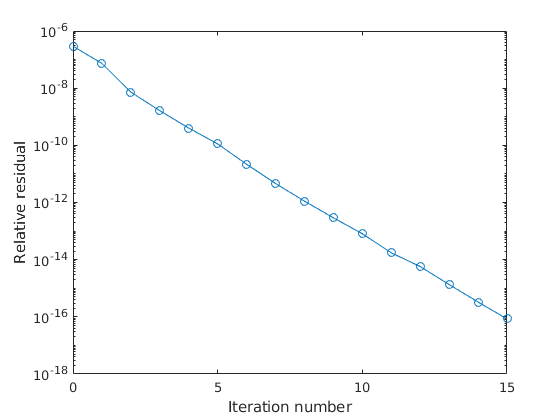
\includegraphics[width=10cm,keepaspectratio]{images/residual_n32.png}
\end{figure}

\pagebreak

\item Consider BVP II with $g=1,\gamma=\eta=\zeta=0$. Exact solution of this BVP is not known. Solve with banded LU and solver from part (a). Output approximate solutions at point (0.5,0.5) of the domain for n=8,16,32,64,128. What is the order of convergence of the computed solutions? How big an n should we take in order to obtain the solution at (0.5,0.5) with $10^{-9}$ precision?\\

\begin{table}[h]
  \begin{center}
    \begin{tabular}{ | c | c | c |}
      \hline
      n & part (a) solver & Banded LU \\
      \hline
      8 & 0.0018806907 & 0.0018806907\\
      \hline
      16 & 0.0019054534 & 0.0019054534\\
      \hline
      32 & 0.0019140108 & 0.0019140108\\
      \hline
      64 & 0.0019163418 & 0.0019163418\\
      \hline
      128 & 0.0019169380 & 0.0019169380\\
      \hline
    \end{tabular}
    \caption{evaluation at (0.5,0.5)}
  \end{center}
\end{table}  

From the previous part, we see PGMRES has an order of convergence of around 2 and the Banded LU solver gives a slightly better answer to the exact solution, meaning it has an order of convergence of 2. Part (a) solver gives an answer that is nearly identical to the Banded LU solver, which is known to have an order of convergence of 2. This means the part (a) solver also has an order of convergence of 2.

Find n for $10^{-9}$ precision at $(0.5,0.5)$:\\

let $v=|u_{16}-u_8|=2.47627*10^{-5}$\\
$\sum_{i=j}^{\infty} v 2^{-2i} \leq 10^{-9}$\\
$\sum_{i=0}^{\infty} (\frac{1}{4})^i - \sum_{i=0}^{j-1} (\frac{1}{4})^i \leq \frac{10^{-9}}{v}$\\
$j \geq -\frac{1}{2}log_2(\frac{3*10^{-9}}{4v}) \approx 7.505$\\
let $j=8$\\
$n=8*2^j=2^{11}$\\

\pagebreak

\begin{verbatim}
ns = [8,16,32,64,128];
for i=1:length(ns)
    n = ns(i);
    dim = n-1;
    g = ones(dim*dim,1);
    fprintf("n: %d\n",n);
    [A, u] = my_precond(n,g);
    mid = n/2;
    k = ij_to_k(dim,mid,mid);
    u_LU = A\g;
    u_mid = u(k);
    u_mid_lu = u_LU(k);
    fprintf("u(midpoint): %.12f\n", u_mid);
    fprintf("LU u(midpoint): %.12f\n", u_mid_lu);
end
\end{verbatim}

\end{enumerate}

\end{enumerate}

\end {document}
